\section{Thiết kế kiến trúc hệ thống}
\label{sec:architecture}

\subsection{Tổng quan kiến trúc}
\label{ssec:arch_overview}

Hệ thống được thiết kế theo mô hình serverless hoàn toàn, tận dụng các dịch vụ được quản lý của AWS để đảm bảo khả năng mở rộng tự động, tính sẵn sàng cao và bảo mật. Kiến trúc tổng thể được minh họa trong Hình \ref{fig:architecture_diagram}.

\begin{figure}[H]
\centering
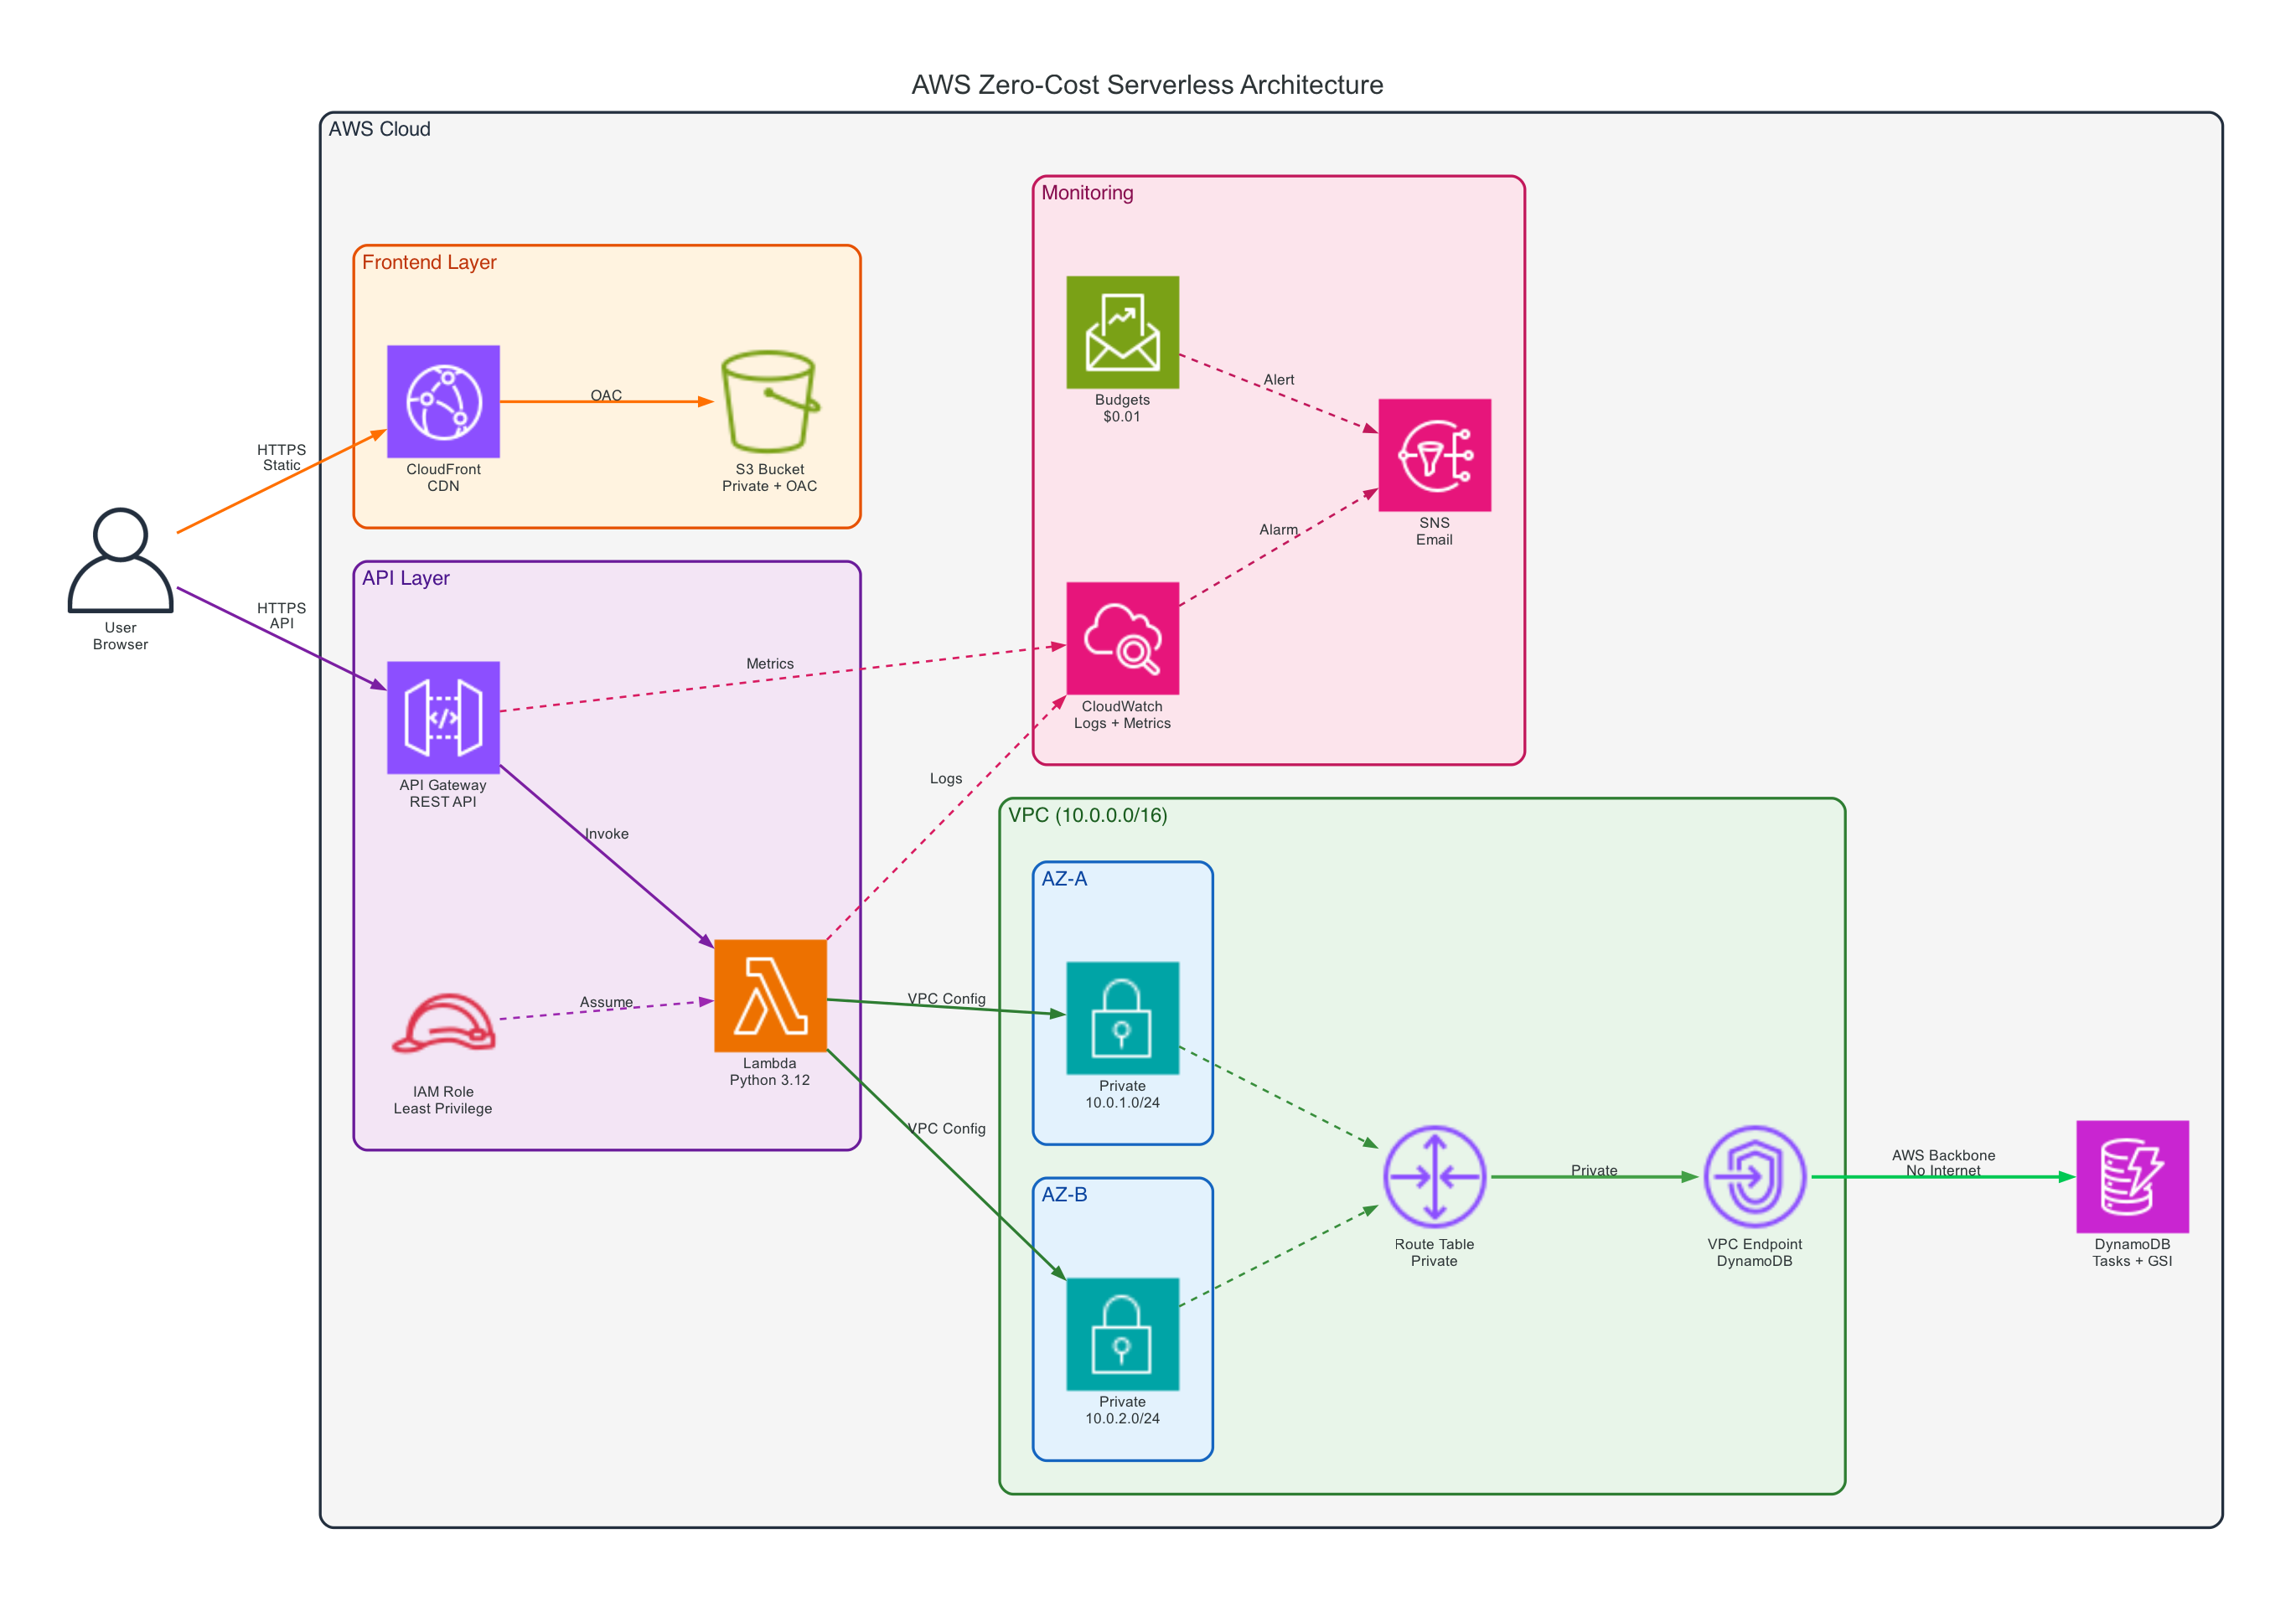
\includegraphics[width=\textwidth]{img/architecture_v3.png}
\caption{Sơ đồ kiến trúc tổng thể của hệ thống}
\label{fig:architecture_diagram}
\end{figure}

Kiến trúc được chia thành các layer chính:

\begin{itemize}
    \item \textbf{Frontend Layer:} CloudFront CDN phục vụ nội dung tĩnh từ S3 bucket private với Origin Access Control (OAC).
    
    \item \textbf{API Layer:} API Gateway nhận request từ client và kích hoạt Lambda function để xử lý logic nghiệp vụ.
    
    \item \textbf{Network Layer:} Custom VPC với 2 Private Subnets trải rộng trên 2 Availability Zones, VPC Gateway Endpoint cho DynamoDB.
    
    \item \textbf{Data Layer:} DynamoDB lưu trữ dữ liệu với Global Secondary Index để truy vấn hiệu quả.
    
    \item \textbf{Monitoring Layer:} CloudWatch, SNS và AWS Budgets để giám sát và kiểm soát chi phí.
\end{itemize}

\subsection{Luồng xử lý request}
\label{ssec:request_flow}

Khi người dùng tương tác với ứng dụng, có hai luồng xử lý chính:

\subsubsection{Luồng truy cập nội dung tĩnh (Static Assets)}

\begin{enumerate}
    \item Người dùng truy cập ứng dụng qua URL CloudFront (https://d1234567.cloudfront.net).
    \item CloudFront kiểm tra cache:
    \begin{itemize}
        \item \textbf{Cache HIT:} Nếu nội dung đã được cache, CloudFront trả về ngay lập tức từ edge location gần nhất, giảm độ trễ và không phát sinh request đến S3.
        \item \textbf{Cache MISS:} Nếu nội dung chưa có trong cache, CloudFront sử dụng Origin Access Control (OAC) để lấy file từ S3 bucket private.
    \end{itemize}
    \item S3 bucket policy chỉ cho phép CloudFront Service Principal đọc objects, từ chối mọi truy cập trực tiếp khác.
    \item CloudFront cache nội dung và trả về cho người dùng qua HTTPS.
\end{enumerate}

\subsubsection{Luồng xử lý API request}

\begin{enumerate}
    \item Người dùng thực hiện thao tác CRUD (ví dụ: tạo task mới) từ giao diện web.
    \item Browser gửi HTTPS request đến API Gateway endpoint (ví dụ: POST /tasks).
    \item API Gateway thực hiện:
    \begin{itemize}
        \item Kiểm tra CORS: Chỉ chấp nhận request từ CloudFront domain.
        \item Áp dụng throttling: Giới hạn 100 requests/second, burst 50 để bảo vệ backend.
        \item Kích hoạt Lambda function tương ứng.
    \end{itemize}
    \item Lambda function được khởi động (cold start nếu chưa có instance sẵn sàng, hoặc warm start nếu đã có):
    \begin{itemize}
        \item Lambda chạy trong VPC, được attach vào 2 Private Subnets (AZ-A và AZ-B) thông qua Elastic Network Interface (ENI).
        \item Lambda sử dụng IAM Role với quyền Least Privilege để truy cập DynamoDB.
    \end{itemize}
    \item Lambda gửi request đến DynamoDB:
    \begin{itemize}
        \item Traffic đi qua VPC Gateway Endpoint (vpce-xxxxx) thay vì Internet.
        \item Route Table của Private Subnets có entry: pl-xxxxx (DynamoDB Prefix List) → vpce-xxxxx.
        \item Security Group của Lambda chỉ cho phép outbound traffic đến port 443 của DynamoDB Prefix List.
        \item Traffic đi hoàn toàn trên AWS backbone network, không ra Internet công cộng.
    \end{itemize}
    \item DynamoDB xử lý request (GetItem, PutItem, UpdateItem, DeleteItem hoặc Query với GSI).
    \item Kết quả được trả về theo đường ngược lại: DynamoDB → VPC Endpoint → Lambda → API Gateway → Browser.
    \item CloudWatch tự động ghi log và metrics của Lambda và API Gateway.
\end{enumerate}

\subsection{Cơ chế Auto-scaling}
\label{ssec:autoscaling}

Một trong những ưu điểm lớn nhất của kiến trúc serverless là khả năng tự động mở rộng mà không cần cấu hình thủ công.

\subsubsection{Lambda Auto-scaling}

AWS Lambda tự động mở rộng theo số lượng request đồng thời:

\begin{itemize}
    \item \textbf{Cold Start:} Khi có request đầu tiên hoặc khi tất cả instances hiện tại đang bận, Lambda tạo một execution environment mới. Quá trình này mất khoảng 100-500ms cho Python runtime.
    
    \item \textbf{Warm Start:} Các request tiếp theo sử dụng lại execution environment đã có, thời gian phản hồi chỉ còn vài milliseconds.
    
    \item \textbf{Concurrent Execution:} Lambda tự động tạo thêm instances khi có nhiều request đồng thời. Mỗi instance xử lý một request tại một thời điểm.
    
    \item \textbf{Reserved Concurrency:} Để kiểm soát chi phí, nhóm đã cấu hình Reserved Concurrency = 50, giới hạn số lượng instances tối đa Lambda có thể tạo ra.
\end{itemize}

\subsubsection{API Gateway Load Balancing}

API Gateway hoạt động như một native load balancer:

\begin{itemize}
    \item Tự động phân phối request đến các Lambda instances khả dụng.
    \item Không cần Application Load Balancer (ALB) riêng biệt.
    \item Hỗ trợ throttling để bảo vệ backend khỏi traffic đột biến.
\end{itemize}

\subsubsection{DynamoDB Auto-scaling}

DynamoDB sử dụng chế độ On-Demand capacity:

\begin{itemize}
    \item Tự động điều chỉnh throughput dựa trên traffic thực tế.
    \item Không cần cấu hình provisioned capacity.
    \item Phù hợp với workload không dự đoán được.
    \item Nằm trong Free Tier: 25 GB storage, 25 RCU/WCU per month.
\end{itemize}

\subsection{High Availability Design}
\label{ssec:high_availability}

Hệ thống được thiết kế để đảm bảo tính sẵn sàng cao mà không cần cấu hình failover thủ công:

\begin{itemize}
    \item \textbf{Multi-AZ Deployment:} Lambda được deploy vào 2 Private Subnets nằm ở 2 Availability Zones khác nhau (ap-southeast-1a và ap-southeast-1b). Nếu một AZ gặp sự cố, Lambda vẫn có thể chạy ở AZ còn lại.
    
    \item \textbf{DynamoDB Multi-AZ Replication:} DynamoDB tự động replicate dữ liệu across multiple AZs trong cùng region, đảm bảo durability 99.999999999\% (11 nines).
    
    \item \textbf{CloudFront Global Edge Network:} CloudFront có hơn 400 edge locations trên toàn cầu, tự động route traffic đến edge location gần nhất và khỏe mạnh nhất.
    
    \item \textbf{API Gateway Regional Endpoint:} API Gateway tự động replicate across AZs trong region.
\end{itemize}

\subsection{Bảo mật theo nguyên tắc Defense-in-Depth}
\label{ssec:security_layers}

Hệ thống áp dụng nhiều lớp bảo mật:

\begin{enumerate}
    \item \textbf{Network Layer:}
    \begin{itemize}
        \item Lambda chạy trong Private Subnets, không có Internet Gateway.
        \item Security Group chỉ cho phép outbound đến DynamoDB Prefix List port 443.
        \item VPC Gateway Endpoint đảm bảo traffic không ra Internet.
        \item Không có NAT Gateway (tránh chi phí \$32/month và giảm attack surface).
    \end{itemize}
    
    \item \textbf{Application Layer:}
    \begin{itemize}
        \item S3 bucket ở chế độ private, tất cả 4 Block Public Access options được bật.
        \item CloudFront OAC đảm bảo chỉ CloudFront mới có thể đọc từ S3.
        \item API Gateway CORS chỉ chấp nhận request từ CloudFront domain cụ thể.
        \item API Gateway throttling bảo vệ khỏi DDoS.
    \end{itemize}
    
    \item \textbf{Identity Layer:}
    \begin{itemize}
        \item Mỗi Lambda function có IAM Role riêng biệt.
        \item IAM Policy áp dụng Least Privilege: chỉ cấp quyền tối thiểu cần thiết.
        \item Resource-based policy: chỉ định chính xác DynamoDB table ARN, không dùng wildcard (*).
    \end{itemize}
    
    \item \textbf{Data Layer:}
    \begin{itemize}
        \item DynamoDB encryption at rest được bật mặc định.
        \item Tất cả traffic đều qua HTTPS/TLS.
    \end{itemize}
\end{enumerate}

\subsection{Chiến lược Zero-Cost}
\label{ssec:zero_cost}

Để đảm bảo chi phí bằng 0, nhóm đã áp dụng các biện pháp sau:

\begin{itemize}
    \item \textbf{Không sử dụng NAT Gateway:} Thay vào đó sử dụng VPC Gateway Endpoint (miễn phí) để Lambda kết nối DynamoDB.
    
    \item \textbf{Lambda Reserved Concurrency = 50:} Giới hạn số lượng instances đồng thời để tránh vượt Free Tier (1 triệu requests/month, 400,000 GB-seconds compute).
    
    \item \textbf{API Gateway Throttling:} Giới hạn 100 req/s, burst 50 để kiểm soát traffic.
    
    \item \textbf{DynamoDB On-Demand:} Nằm trong Free Tier: 25 GB storage, 25 RCU/WCU.
    
    \item \textbf{CloudFront Free Tier:} 1 TB data transfer out, 10 triệu HTTP/HTTPS requests.
    
    \item \textbf{S3 Free Tier:} 5 GB storage, 20,000 GET requests, 2,000 PUT requests.
    
    \item \textbf{AWS Budgets:} Cấu hình budget \$0.01 với alerts ở 80\% và 100\% để phát hiện sớm nếu có chi phí phát sinh.
\end{itemize}
